\documentclass[10pt, a4paper]{article}
\usepackage[a4paper, top=20mm, left=18mm, right=18mm, bottom=20mm]{geometry}
\usepackage{hyperref}
\usepackage[sf]{titlesec}
\usepackage{listings}
\usepackage{graphicx}
\usepackage{float}
\usepackage{color}
\hypersetup{hidelinks = true}
\definecolor{codegrey}{rgb}{0.95, 0.95, 0.96}
\lstset{backgroundcolor = \color{codegrey}}

\begin{document}
{\fontfamily{cmss}\selectfont

\title{\vspace{-20mm}CMPUT 291 - Mini Project 2 Design Document}
\date{}
\maketitle
\vspace{-20mm}

\section{Overview}\label{OV}
The following software package is cmprosed of 3 phases. Phase 1 takes email data from an XML file and outputs the data into four files: terms.txt, emails.txt, dates.txt, and recs.txt. Phase 2 sorts these files and builds four indexes. Phase 3 is responsible for data retrival, and queries the data.

\begin{figure}[H]
\centering
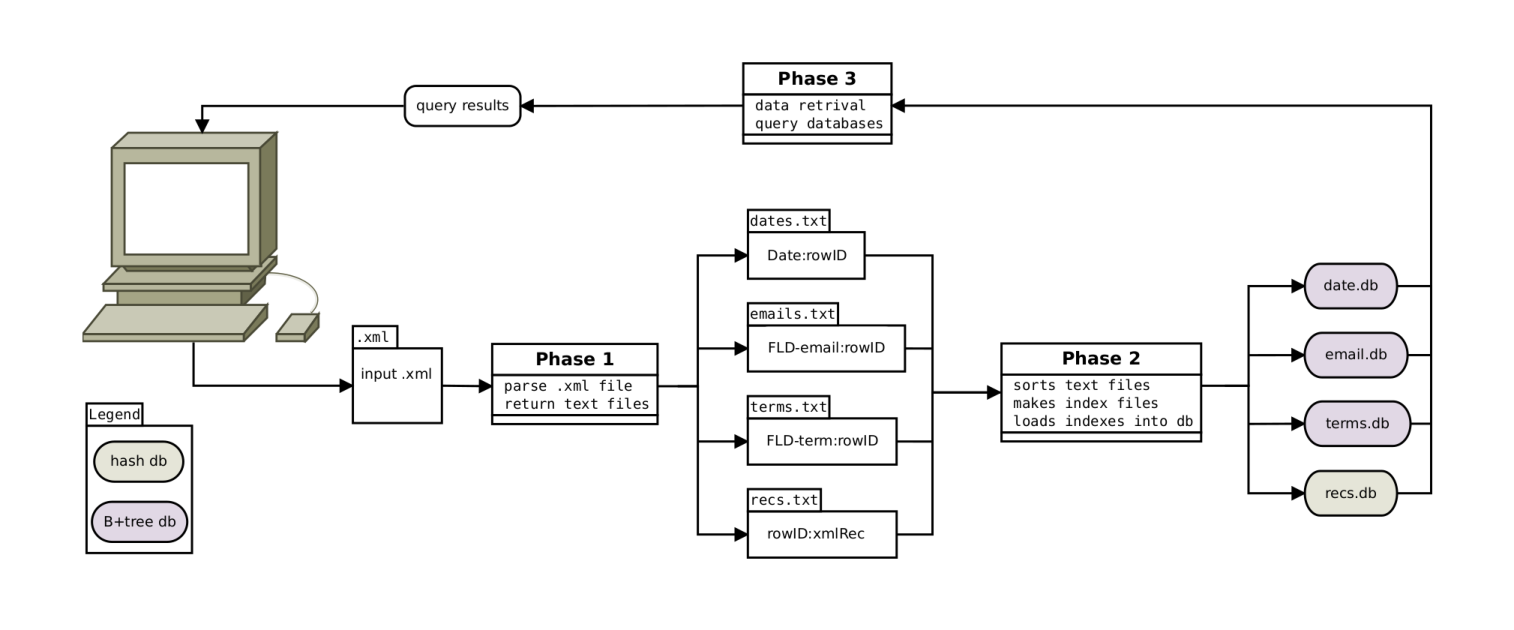
\includegraphics[width = \textwidth]{software_FD.pdf}\label{fig}
\caption{Flow diagram of files, data, and different phases of the software. For more implementation details see \emph{\nameref{SD}}.}
\end{figure}

\subsection{User Guide}\label{UG}

\subsubsection{Phase 1: Preparing Data Files}
The software for phase 1 is a python program that reads email records in an XML file and prodcues four output files: terms.txt, emails.txt, dates.txt, and recs.txt. To run phase 1, execute the program in the terminal
\begin{lstlisting}
    $ python3 phase1.db
\end{lstlisting}
The program will propmt the user to enter an XML file.
\begin{lstlisting}
    Enter .xml file: datafile.xml
\end{lstlisting}
If the provided file is not found, or an incorrect file extension is given, an error message will display, and the user can re-enter a filename. If no extension is specified, the program will assume it is .xml.

When a valid file is entered, phase 1 parses the XML file into the four text files mentioned above. If those files already exist in the directory, the program will overwrite the data currently on the files.

\subsubsection{Phase 2: Building Indexes}

\subsubsection{Phase 3: Data Retrieval}

\section{Software Design}\label{SD}

\end{document}
